\begin{answer}
    \begin{figure}[htbp]
        \begin{subfigure}[b]{0.5\linewidth}
            \centering
            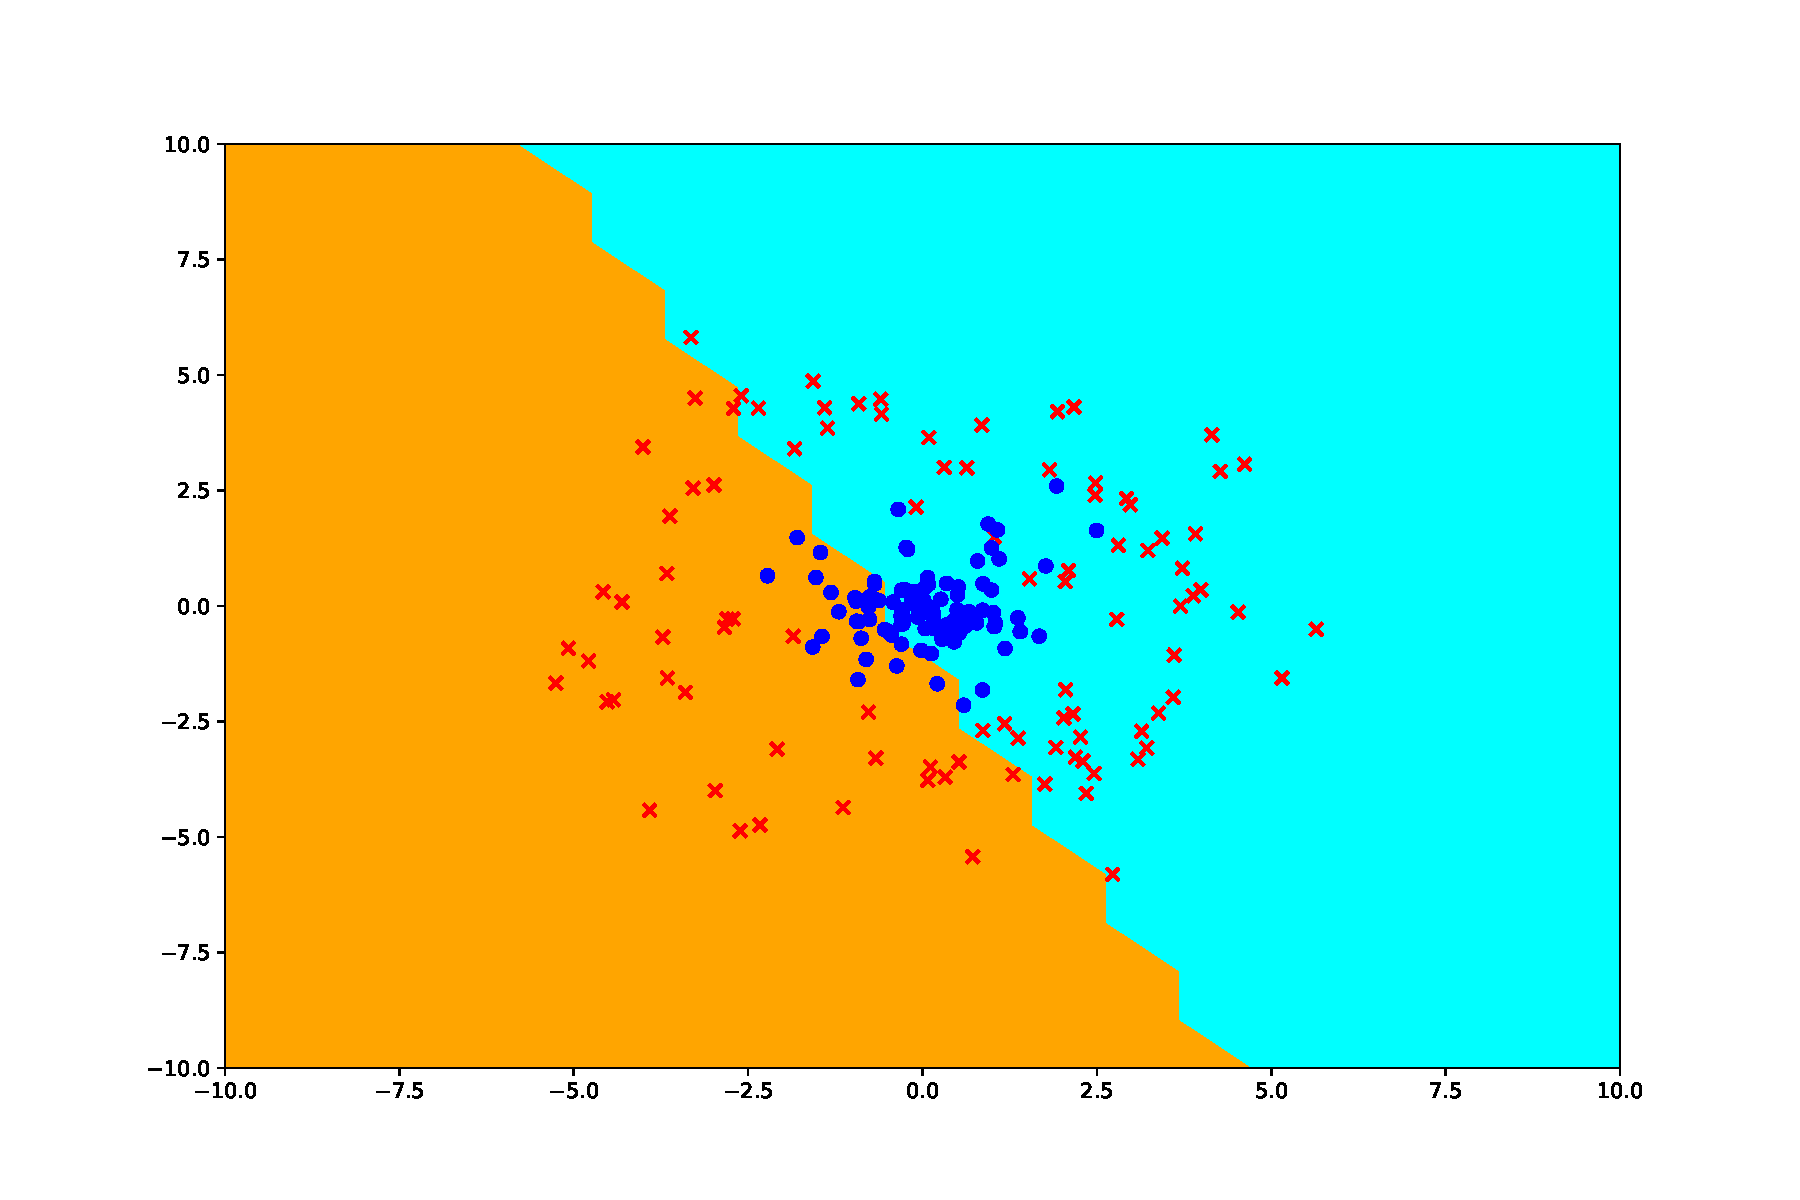
\includegraphics[width=\linewidth]{pics/p05_dot_output.pdf}
            \caption{Dot}
        \end{subfigure}
        \begin{subfigure}[b]{0.5\linewidth}
            \centering
            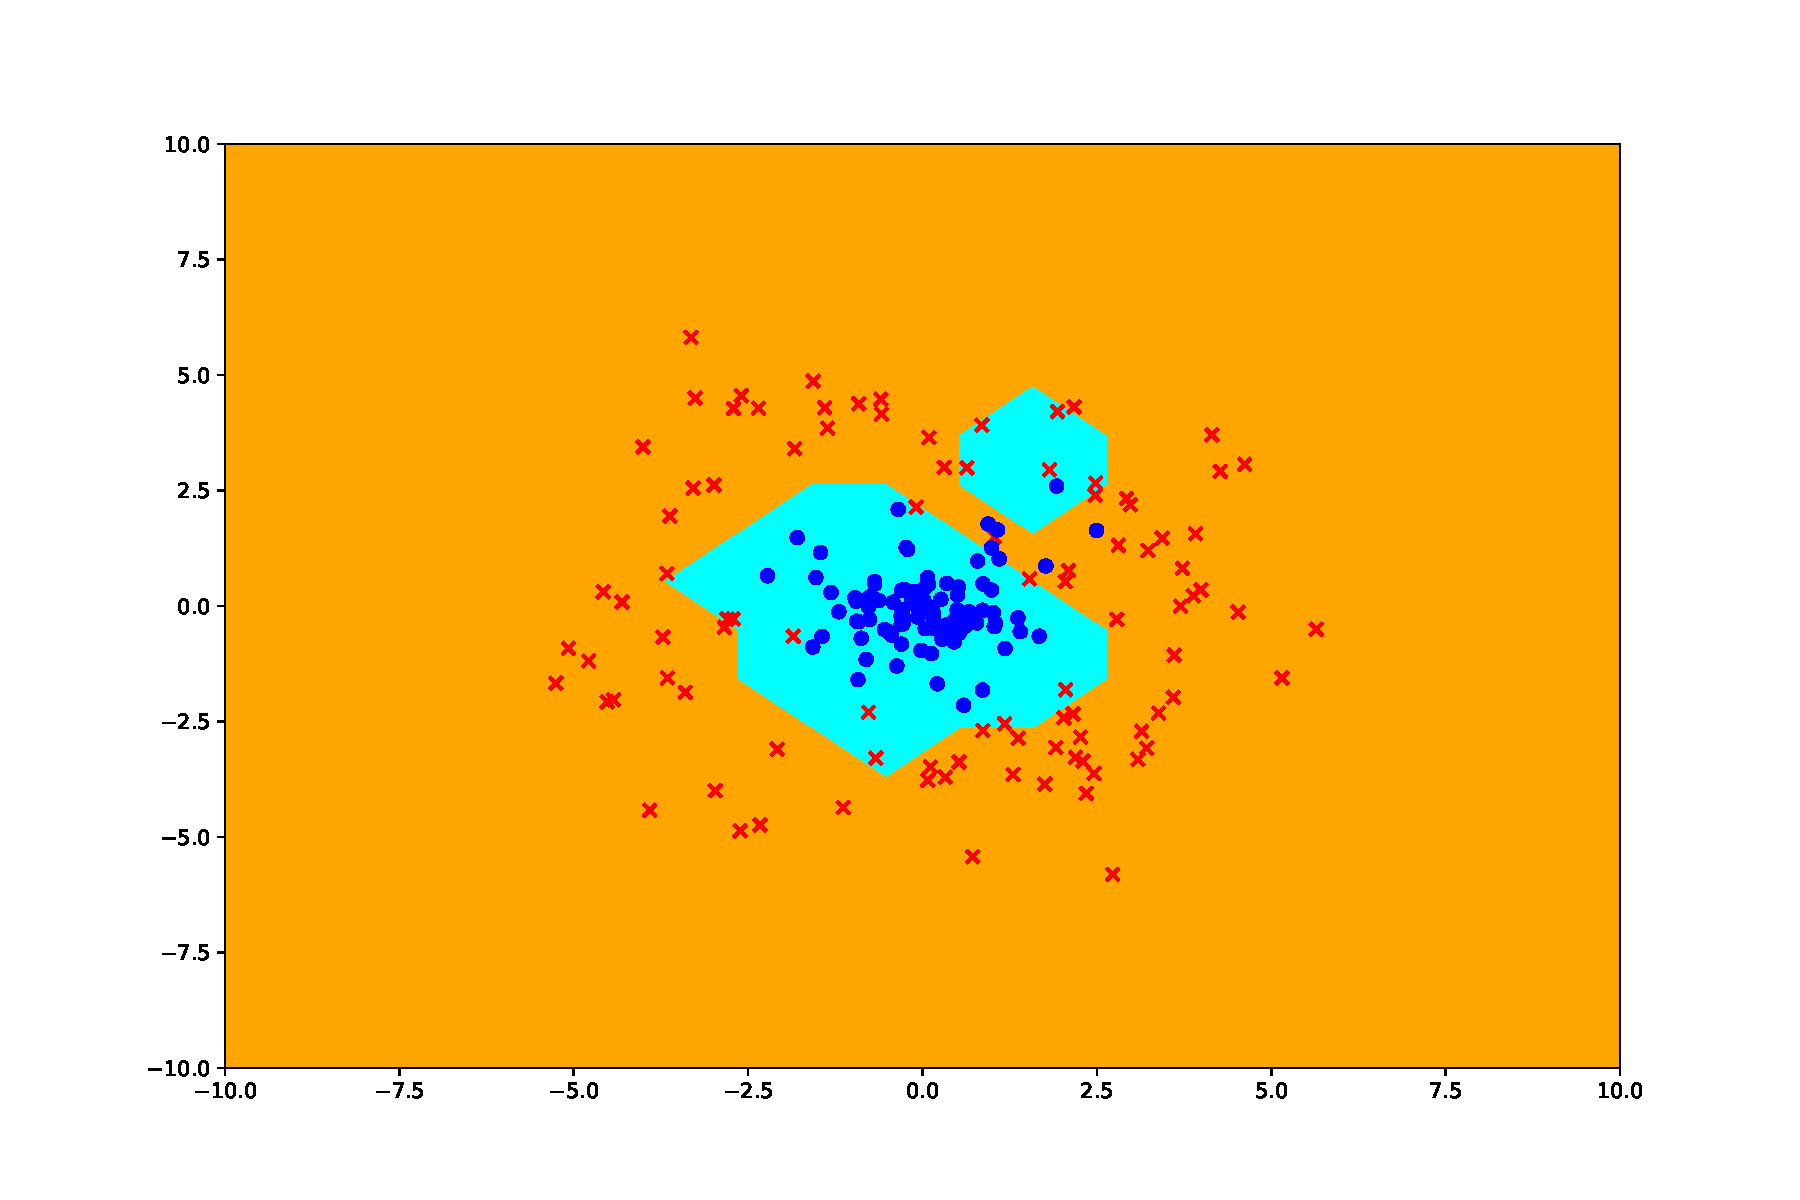
\includegraphics[width=\linewidth]{pics/p05_rbf_output.pdf}
            \caption{RBF}
        \end{subfigure}
    \end{figure}

    The fist performs poorly because using dot product it is equivalent to use $\phi(x^{(i)}) = x^{(i)}$, but the data is not linearly seperable.
\end{answer}
